\chapter{Projeto proposto: Enriquecimento de contexto de entidades no tempo}

Tendo agora explorado de maneira relativamente detalhada as diferentes etapas do sistema completo proposto por este trabalho, podemos isolar algumas partes e focar em alguns detalhes de implementação da etapa de enriquecimento de contexto que imaginamos ser cruciais para o alcance de resultados excelentes na modelagem de contexto semântico propriamente dita.

\section{Metodologia}

Serão descritas duas abordagens, ambas sujeitas a todas as etapas do sistema completo exceto a de enriquecimento de contexto: \textbf{coleta} de múltiplas fontes de dados; \textbf{processamento} de múltiplas camadas de dados; e \textbf{aplicação} do conhecimento extraído em recomendação de conteúdo e agentes virtuais. 

\begin{itemize}
    \item Consideraremos como \textbf{abordagem clássica}, aquela que faz uso de apenas um tipo de canal de dados por vez durante a aplicação, pois não contempla uma camada de enriquecimento multidimensional de contexto.
    \item  Por outro lado, descrevemos como \textbf{abordagem multidimensional} aquela que faz uso de todas as técnicas descritas no capítulo \ref{c:enriquecimento_de_contexto} para fornecer uma definição de contexto rica à camada de aplicação.
\end{itemize}

Espera-se ser possível identificar com facilidade a fragilidade da \textbf{abordagem clássica} e os benefícios da \textbf{abordagem multidimensional} a partir dos modelos expostos neste capítulo.

\newpage

\section{Fluxo de processamento}

O fluxo de processamento, em cada um dos cenários, é representado a seguir:

\begin{figure}[h]
\caption{abordagem clássica}
\centering
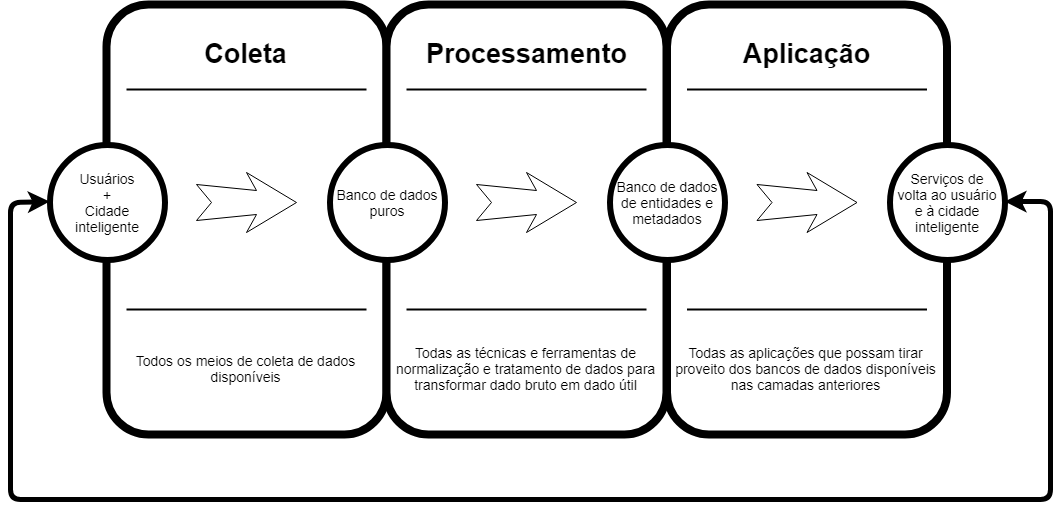
\includegraphics[width=0.8\textwidth]{images/PoorFlow.png}
\end{figure}

\begin{figure}[h]
\caption{abordagem multidimensional}
\centering
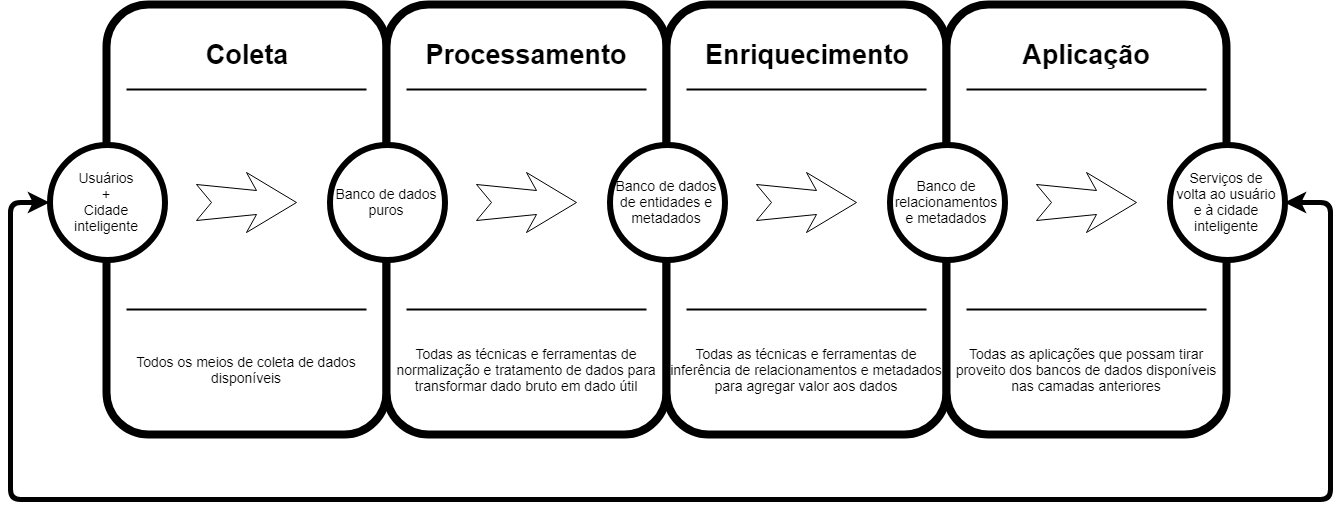
\includegraphics[width=0.8\textwidth]{images/FullFlow.png}
\end{figure}

\section{Estrutura das representações de contexto}

Apesar dos detalhes das etapas do fluxo terem sido descritas anteriormente, a camada de aplicação pode ser considerada agnóstica quanto à implementação dos bancos de dados de entidades, metadados e relacionamentos. Com isso, podemos considerar que a estrutura da representação de contexto de cada um dos cenários confia nas camadas anteriores de maneira transparente.

\newpage

\begin{minted}[
    frame=lines,
    framesep=2mm,
    baselinestretch=0.8,
    fontsize=\footnotesize,
    linenos
]{groovy}
/**
* Defines a single relationship between a document/event and an entity.
* Contains as much metadata as available in the original event
*/
class SD_EntityEventRelationship {
    //mandatory, identifies the data content that generated this relationship
    Event originalEvent
    //mandatory, points to a definition of an entity on an Ontology/Thesaurus
    Entity entity

    //timestamp is so common that we can consider the SD model to have it,
    //but it isn't properly used in the query process
    //optional, with as much precision as possible
    Timestamp timestamp
}

/**
* Defines the query used in a context
* to search for all possible entityEventRelationships,
* in the single-dimension scenario,
* and without considering an oerall multilayered context.
* Note that this match only cares for the {entity} relation:
* it's unaware of time or place, or any other metadata
*/
class SD_ContextQuery {
    Entity entity
}

/**
* Defines the answer to a SD_ContextQuery
*/
class SD_ContextualMatch {
    //this contains all occurencies of the matched entity
    List<EntityEventRelationship> matchHistory

    /**
    * calculated from the distance between the query entity
    * and the matched EntityEventRelationship
    */
    BigDecimal relevance
}
\end{minted}

Blablabla blablabla

\newpage


\begin{minted}[
    frame=lines,
    framesep=2mm,
    baselinestretch=0.8,
    fontsize=\footnotesize,
    linenos
]{groovy}
/**
* Augments the original EntityEventRelationship with all the other
* metadata layers
*/
class MD_EntityEventRelationship extends SD_EntityEventRelationship {
    
    //now mandatory, most of the time with a millisecond precision
    Timestamp timestamp
    //now mandatory, with as much precision as possible
    Coodinates coordinates
    //optional, freeform metadata that doesn't fit time or place concepts
    HashMap extraMetadata

    /**
    * Instead of having simple and single entityEventRelationships,
    * we can provide the API with a way to inspect all neighbours
    * of the one that triggered the match, which will paint
    * the picture of the whole rich original context
    * of all the channels collecting data
    */
    public List<MD_EntityEventRelationship> nearbyEntityEventRelationships() {
        /*...*/
    }
}

/**
* Represents a cluster of EntityEventRelationship that are
* near each other in at least one dimension/attribute.
*
* We can represent this as a cloud of events that have a high
* temporal/georeferencial/semantic relationship between them
*/
class MD_CompositeContextSurface {
    HashMap<MD_EntityEventRelationship, Point> surface
}

/**
* The same as SD_ContextQuery,
* but taking into account all available metadata
*/
class MD_ContextQuery {
    Entity entity

    Timestamp timestamp
    Coodinates coordinates
    HashMap extraMetadata
}

class MD_ContextualMatch {
    //this contains all occurencies of the matched query on all layers and dimensions
    List<MD_CompositeContextSurface> matchHistory

    /**
    * calculated from the collective distance between all attributes
    * of the query and the MD_CompositeContextSurface
    * 
    * a list of distances of each attribute could also be implemented,
    * to supply queries targeted on a single domain, like time
    */
    BigDecimal relevance
}
\end{minted}

Blablabla blablabla

\newpage
